\section{Maps}
\label{app:maps}

Figure~\ref{fig:appendix-bvr-treatment-map} maps the municipal rollout of biometric registration by first observed BVR year, including municipalities observed with hybrid status. The figure complements the rollout timeline in the main text by showing the spatial concentration of later BVR waves and the municipalities flagged as hybrid in the official 2018 status source.

\begin{figure}[p]
    \caption{Municipal Biometric Registration Rollout by First Treatment Year}
    \label{fig:appendix-bvr-treatment-map}
    \centering
    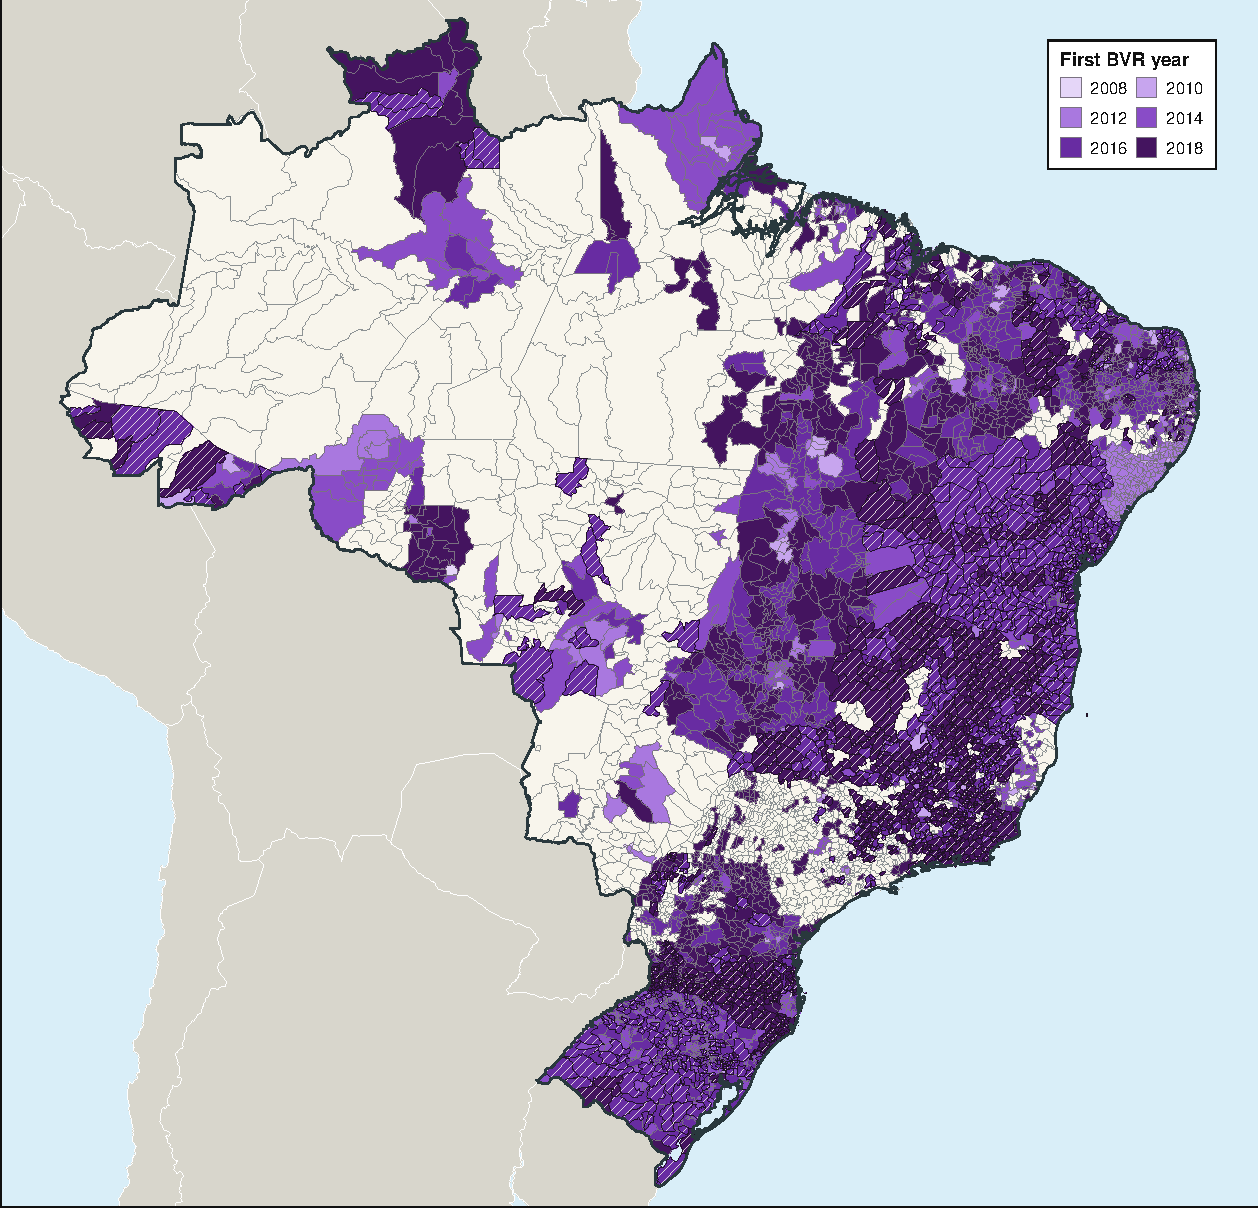
\includegraphics[width=0.9\textwidth]{../resources/maps/brazil_municipalities_bvr_treatment_year.pdf}
    \vspace{0.75em}
    \begin{minipage}{\textwidth}
        {\footnotesize \textbf{Note:} Municipalities are shaded by the first election year in which they are observed with any BVR status, including hybrid implementation. Unshaded municipalities have no observed BVR status through 2018 in the clean municipal panel. Diagonal hatching identifies municipalities flagged as hybrid in the official 2018 biometric-status source. The map uses the 2010 IBGE municipal geometry, so municipalities absent from that shapefile are not drawn. \par}
    \end{minipage}
\end{figure}
